%!TEX root = ../../thesis.tex
Soft robotics is an established scientific field that explores continuum elastic robots. Through its high-elasticity, intrinsic motion and adaptability can be achieved in ways previously unseen in rigid robotics. Although this leads to robots with beneficial properties,it homogeneous structural elasticity imposes challenge on modeling and control. The introduction of elastic structures has lead to a new paradigm shift regarding robotics control theory \cite{DellaSantina2021}; namely, feedback regularization of (underactuated) deformable robots with theoretically infinite-dimensional Degrees-of-Freedoms (DOFs). Although this problem has an inception earlier than origin of soft robotics (\eg, \cite{Chirikjian1991,DeLuca2016Jul}), it remains challenging ever since.

As of today, two dynamic modeling strategies lead control community in soft robotics with clear direction for model-based control: \textit{(i)} Finite-Element-Method (FEM) models and \textit{(ii)} soft beam models. FEM is a well-known technique which employs spatial discretization to Partial Differential Equations (PDEs) such that their approximates can be solved numerically \cite{Bonet2016,Holzapfel2002,Kim2018}. Deeply rooted in continuum mechanics, FEM is a matured field that, through mesh discretization and its local deformation, easily incooperates constitutive material laws, nonlinear geometric deformations, and multi-physics interactions. However, high-accuracy FEM requires fine mesh discretization that severely impacts computational cost, \ie, $\mathcal{O}(n^3)$ for increasing mesh sizes. This renders online state estimation and feedback control often infeasible for the original system. To enable feedback strategies, several model reduction strategies have been proposed, \eg, Proper-Orthogonal-Decomposition \cite{Coevoet2017,Duriez2013,Goury2018,Thieffry2017} or iterative Krylov reduction, in which the configuration space (\ie, nodal displacements) is projected onto an optimal subspace. Yet, to be enable these subspace projection, soft robot models are often linearized to produce a linear time-invariant systems (LTI), which leads to controllers with local stability guarantees \cite{Thieffry2017,Goury2018,Katzschmann2019}. In some recent works, however, researchers have extended to nonlinear projections \cite{Chenevier2018}, or linear-parameter varying systems (LPV) \cite{Thieffry2020}. Although promising, perhaps even leading the field on experimental basis, it is challenging to preserve desirable system properties, \eg, passivity or physical state interpretation useful for sensor placement.

Contrary, soft beam models, like the (non)-constant curvature \cite{Katzschmann2019,DellaSantina2020,Caasenbrood2022} and Cosserat beams \cite{Boyer2021,Renda2020}, have roots in Lagrangian-based modeling principles. By predefining a minimal joint representation, reduced-order ODE systems are formulated akin to the traditional models for (serial-elastic) rigid robots. Consequently, it enables a rich collection of pre-existing control theory adopted from rigid robotics: computed-torque control \cite{Katzschmann2019}, back-stepping \cite{Stolzle2021}, passivity-based (adaptive) control \cite{Caasenbrood2022,Franco2020}, and swing-up controllers \cite{Weerakoon2021Dec}. Here the continuum dynamics of the soft robot are modeled as spatial elastic strings; whose time-varying deformation is either described through discrete links along the arc-length, or functional parameterization. These models trade the description for volumetric deformations for low-dimensionality (and thus computation speed). In doing so, the method loses many geometric features of the soft robot's morphology and its coupling to actuation (\eg, tendons, pneumatics). Consequently, many of the physical properties such as the stiffness, damping, and actuation mapping are lost in favor of minimal model complexity. The modeling technique demands empirical matching between model and \emph{a-priori} experimental data, which is often time-consuming and tedious compared to standard FEM.

\begin{figure}[!t]
  \ifx\printFigures\undefined
  \else
  \centering
  \input{./3_chapters/4_chapter/img/fig_pneunet.tex}
  \vspace{1mm}
  \fi
  \caption{(a) PneuNet bending actuator composed of DragonSkin 10 silicone rubber wrapping around an aluminum rod of radius $r = 10 \,\si{\milli \meter}$. The actuator is subjected to an input of $u = 30 \si{\kilo \pascal}$. (b) FEM model of bending PneuNet simulated using the \sorotoki toolkit. }
  \label{fig:C4:pneunet}
  \vspace{-5mm}
\end{figure}

\textbf{Problem description}: Let us discuss the problem into more detail. To help clarify the problem, consider a silicone \textit{PneuNet} actuator as shown in Figure \ref{fig:C4:pneunet} inspired by Mosadegh et al. (2014, \cite{Mosadegh2014}). When pressurized, the volumetric expansion of the soft actuator causes a uniform bending motion, allowing thest soft actuators for \textit{adaptive grasping} (see Figure \ref{fig:C4:pneunet}). Yet, in part due to hyper-elasticity, structural complexity, and distributed actuation, these systems are rarely considered in control-oriented research. This motivates our work here to develop a compact soft beam model, capable of describing such behavior with sufficient accuracy and speed suited for real-time control. In many cases, FEM is preferred over beam models since it is unclear \textit{a-priori} how structural geometry will affect displacement. To highlight its precision, Figure \ref{fig:C4:pneunet} shows a FEM simulation of the bending PneuNet grasping a cylinder of radius $r = 10 \, \si{\milli \meter}$ produces using the \sorotoki  toolkit. Although accurate, such dynamic simulations are often time-consuming. In this case, the dynamic simulation of the grasping PneuNet took about $T_\textrm{sim} \approx 5 \,\si{\minute}$ for a $T = 2 \,\si{\second}$ horizon time given about 6k Degrees-of-Freedom.
% %
% \begin{figure}[!t]
%   \ifx\printFigures\undefined
%   \else
%   \centering
%   \vspace{-5mm}
%   % This file was created by matlab2tikz.
%
%The latest updates can be retrieved from
%  http://www.mathworks.com/matlabcentral/fileexchange/22022-matlab2tikz-matlab2tikz
%where you can also make suggestions and rate matlab2tikz.
%
\definecolor{mycolor1}{rgb}{0.90627,0.93569,0.98471}%
\definecolor{mycolor2}{rgb}{0.71882,0.80706,0.95412}%
\definecolor{mycolor3}{rgb}{0.53137,0.67843,0.92353}%
\definecolor{mycolor4}{rgb}{0.34392,0.54980,0.89294}%
\definecolor{mycolor5}{rgb}{0.15647,0.42118,0.86235}%
\definecolor{mycolor6}{rgb}{0.06275,0.35686,0.84706}%
\definecolor{mycolor7}{rgb}{0.98667,0.92118,0.91098}%
\definecolor{mycolor8}{rgb}{0.96000,0.76353,0.73294}%
\definecolor{mycolor9}{rgb}{0.93333,0.60588,0.55490}%
\definecolor{mycolor10}{rgb}{0.90667,0.44824,0.37686}%
\definecolor{mycolor11}{rgb}{0.88000,0.29059,0.19882}%
\definecolor{mycolor12}{rgb}{0.86667,0.21176,0.10980}%
\definecolor{mycolor13}{rgb}{0.91804,0.95216,0.92510}%
\definecolor{mycolor14}{rgb}{0.75412,0.85647,0.77529}%
\definecolor{mycolor15}{rgb}{0.59020,0.76078,0.62549}%
\definecolor{mycolor16}{rgb}{0.42627,0.66510,0.47569}%
\definecolor{mycolor17}{rgb}{0.26235,0.56941,0.32588}%
\definecolor{mycolor18}{rgb}{0.18039,0.52157,0.25098}%
%
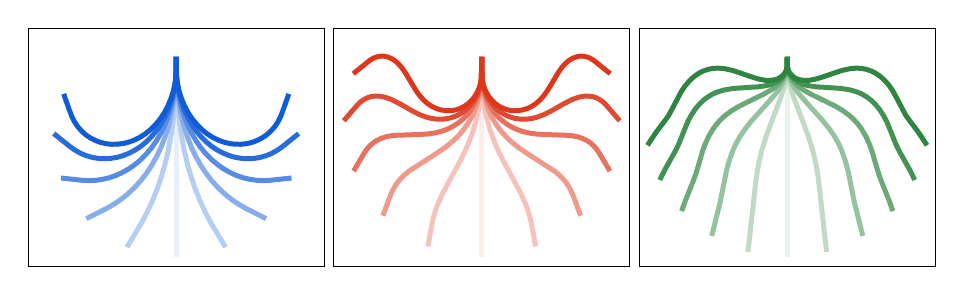
\begin{tikzpicture}

\begin{axis}[%
width=0.31\textwidth,
height=0.25\textwidth,
at={(0\textwidth,0\textwidth)},
scale only axis,
xmin=-80,
xmax=80,
xtick={\empty},
ymin=-110,
ymax=15,
ytick={\empty},
axis background/.style={fill=white},
xmajorgrids,
ymajorgrids
]
\addplot [color=mycolor1, line width=1.8pt, forget plot]
  table[row sep=crcr]{%
-0	-0\\
-3.74110697975993e-09	-105.000000000093\\
};
\addplot [color=mycolor2, line width=1.8pt, forget plot]
  table[row sep=crcr]{%
-0	-0\\
-0.161167305614711	-14.6979016016311\\
-0.724205215537552	-24.130440948486\\
-1.62484165251422	-33.0092288329655\\
-2.84391219608735	-41.3196183063557\\
-4.33983286239373	-49.050450688916\\
-6.08370480837714	-56.1898067668033\\
-8.02329978269697	-62.732687217309\\
-10.2880396765699	-69.1701626624276\\
-12.8963845981263	-75.4762175116649\\
-15.6125943796508	-81.1598503440699\\
-18.6249257861769	-86.6921487779278\\
-22.7290512138719	-93.4126180754324\\
-26.6259047319698	-99.6445592329526\\
};
\addplot [color=mycolor2, line width=1.8pt, forget plot]
  table[row sep=crcr]{%
-0	-0\\
0.16116730531246	-14.6979016016379\\
0.724205214637607	-24.130440948529\\
1.62484165100592	-33.0092288330701\\
2.84391219406344	-41.3196183065356\\
4.33983285997653	-49.0504506891717\\
6.08370480568817	-56.1898067671251\\
8.02329977979984	-62.7326872176925\\
10.2880396734375	-69.1701626628943\\
12.8963845946628	-75.4762175122693\\
15.6125943757099	-81.1598503449036\\
18.6249257815266	-86.6921487791495\\
22.729051208088	-93.4126180773471\\
26.6259047251041	-99.6445592355437\\
};
\addplot [color=mycolor3, line width=1.8pt, forget plot]
  table[row sep=crcr]{%
-0	-0\\
-0.177893259763749	-12.5966006933054\\
-0.722799877549349	-18.8723054652083\\
-1.6172652219318	-25.1077882322473\\
-2.86723713149574	-31.2817043271525\\
-4.35520972922873	-36.8608837669467\\
-6.00297555696973	-41.8447342667065\\
-8.15281158930638	-47.2032533564516\\
-10.4412041132732	-51.9271256234893\\
-13.3337988131099	-56.9240309154601\\
-16.3102592374528	-61.2475676850593\\
-19.2709663978063	-64.9286256660791\\
-22.494132356736	-68.3818183271243\\
-26.3674110900965	-71.9236914008764\\
-30.1069489334551	-74.8103679944717\\
-33.6152947038996	-77.1176148946514\\
-37.7381561765432	-79.423727386133\\
-48.1109470243421	-84.5036653552529\\
-48.5829593109394	-84.7335144535623\\
};
\addplot [color=mycolor3, line width=1.8pt, forget plot]
  table[row sep=crcr]{%
-0	-0\\
0.177893259565565	-12.5966006933118\\
0.722799877003339	-18.8723054652452\\
1.61726522096534	-25.1077882323446\\
2.8672371301023	-31.2817043273363\\
4.35520972747106	-36.8608837672274\\
6.00297555491923	-41.844734267084\\
8.15281158698366	-47.203253356938\\
10.4412041107574	-51.9271256240689\\
13.3337988104245	-56.9240309161376\\
16.3102592346297	-61.2475676858315\\
19.270966394848	-64.9286256669605\\
22.4941323536211	-68.3818183281525\\
26.3674110867562	-71.9236914021522\\
30.1069489298487	-74.8103679960935\\
33.6152947000067	-77.1176148967104\\
37.7381561722927	-79.423727388833\\
48.1109470192074	-84.5036653597581\\
48.5829593057649	-84.7335144581494\\
};
\addplot [color=mycolor4, line width=1.8pt, forget plot]
  table[row sep=crcr]{%
-0	-0\\
-0.150304668408126	-11.021676549763\\
-0.615047720310358	-15.7227967673249\\
-1.4730458810207	-20.9010846925926\\
-2.83239088840696	-26.5125449229663\\
-4.45576347512329	-31.5042921035373\\
-6.25997987798416	-35.8702342255958\\
-8.37910677923186	-40.0917972793852\\
-10.8203429289321	-44.1360000958585\\
-13.6113768299572	-47.9470892087042\\
-16.3809566877961	-51.1026808938959\\
-19.3970302670867	-54.023792212002\\
-22.6705460127614	-56.6534408652387\\
-25.7180062261556	-58.7053274633946\\
-29.3992060929905	-60.7248374310415\\
-32.7779204776504	-62.1677186337703\\
-36.2641435834314	-63.3268177998917\\
-39.8456657780698	-64.1458788202489\\
-43.484615378102	-64.6499599756908\\
-47.1557596767798	-64.7965094636445\\
-50.8260913119345	-64.6328067054671\\
-61.7921541973648	-63.4948917144393\\
-62.3142279171542	-63.4395126764606\\
};
\addplot [color=mycolor4, line width=1.8pt, forget plot]
  table[row sep=crcr]{%
-0	-0\\
0.150304668273776	-11.0216765497678\\
0.61504771995061	-15.7227967673526\\
1.4730458803411	-20.9010846926736\\
2.8323908873431	-26.5125449231404\\
4.45576347371512	-31.5042921038232\\
6.2599798762898	-35.8702342259998\\
8.37910677728618	-40.0917972799153\\
10.8203429267716	-44.136000096518\\
13.6113768276226	-47.9470892094907\\
16.3809566853418	-51.1026808947874\\
19.3970302645367	-54.0237922129921\\
22.6705460101274	-56.6534408663334\\
25.7180062234527	-58.7053274645918\\
29.3992060902059	-60.724837432388\\
32.7779204747929	-62.1677186352885\\
36.2641435804996	-63.3268178016343\\
39.8456657750681	-64.1458788222998\\
43.484615375046	-64.6499599781394\\
47.1557596737039	-64.7965094666048\\
50.8260913088855	-64.6328067090194\\
61.7921541945141	-63.4948917199021\\
62.314227914313	-63.4395126820139\\
};
\addplot [color=mycolor5, line width=1.8pt, forget plot]
  table[row sep=crcr]{%
-0	-0\\
-0.158714240849918	-10.4957380689595\\
-0.643456607656773	-14.6664630646084\\
-1.56177730776834	-19.3003428573835\\
-2.87329104506745	-23.8385656398972\\
-4.35366906790726	-27.7677103873271\\
-6.38065329246329	-32.0342062552411\\
-8.53471518723688	-35.6387537959117\\
-10.6698902899409	-38.62839593889\\
-13.3962472900377	-41.8218435722855\\
-16.042764298039	-44.3697360597515\\
-18.9045077376541	-46.6734920762282\\
-21.9894665098523	-48.6687249219677\\
-25.2474957894325	-50.3651818383069\\
-28.6707971367788	-51.6986217782939\\
-31.7009666001305	-52.5548076811513\\
-35.3228121857963	-53.1695904027016\\
-38.4656121153509	-53.3581056467778\\
-42.1351076635131	-53.1829307696389\\
-45.2430470350136	-52.6791209463755\\
-48.7813032393877	-51.6916161375571\\
-51.6953179082226	-50.4996026624502\\
-54.9151796725102	-48.7311563693139\\
-57.9207488268187	-46.6184639367124\\
-66.1937276697712	-40.1524535624561\\
};
\addplot [color=mycolor5, line width=1.8pt, forget plot]
  table[row sep=crcr]{%
-0	-0\\
0.158714240734739	-10.4957380689643\\
0.64345660735593	-14.6664630646354\\
1.56177730719449	-19.3003428574648\\
2.87329104418585	-23.8385656400675\\
4.35366906675364	-27.7677103876\\
6.38065329102	-32.0342062556515\\
8.53471518555983	-35.6387537964616\\
10.6698902880861	-38.6283959395667\\
13.3962472880089	-41.8218435731105\\
16.0427642958861	-44.3697360607052\\
18.9045077354067	-46.6734920772989\\
21.9894665075315	-48.6687249231518\\
25.2474957870576	-50.3651818395947\\
28.6707971343612	-51.6986217796914\\
31.7009665976848	-52.5548076826488\\
35.3228121833263	-53.1695904043426\\
38.4656121128726	-53.3581056485625\\
42.1351076610453	-53.182930771638\\
45.2430470325837	-52.6791209486046\\
48.7813032370528	-51.6916161401245\\
51.6953179060312	-50.4996026653665\\
54.9151796705779	-48.7311563727008\\
57.9207488252398	-46.6184639406011\\
66.193727669319	-40.1524535677865\\
};
\addplot [color=mycolor6, line width=1.8pt, forget plot]
  table[row sep=crcr]{%
-0	-0\\
-0.151941493802298	-9.97038329054241\\
-0.702860123201781	-14.1323325814535\\
-1.65361201498619	-18.2223483966822\\
-2.79949575649412	-21.7129392628167\\
-4.43546427070452	-25.5798217214961\\
-6.45250301160665	-29.2622500793775\\
-8.5118695864172	-32.3039651278895\\
-11.2089060035391	-35.5218867085713\\
-13.8628395505385	-38.0616063696407\\
-16.7486191859941	-40.3349866392992\\
-19.4230535106411	-41.9970510342485\\
-22.7232482558487	-43.6097075139492\\
-25.6998614648023	-44.637175497262\\
-28.7605771895863	-45.3760789932858\\
-31.8879766612167	-45.7407803418752\\
-35.0365074933738	-45.7763301351314\\
-38.1643228962581	-45.4187994208609\\
-41.2306386247369	-44.7036209787197\\
-43.6917729830663	-43.7939406630027\\
-46.5115024599121	-42.3926099459278\\
-48.7039018400521	-40.9512728403363\\
-51.1047024855009	-38.9141858812766\\
-53.2313868091573	-36.5935732423494\\
-55.0079531829889	-33.9943211134134\\
-56.4615464620177	-31.2018334865171\\
-57.9804093930198	-27.2867324414782\\
-60.8405264008306	-19.3885089291719\\
};
\addplot [color=mycolor6, line width=1.8pt, forget plot]
  table[row sep=crcr]{%
-0	-0\\
0.151941493705358	-9.97038329054687\\
0.702860122929252	-14.1323325814818\\
1.65361201447916	-18.2223483967652\\
2.79949575575692	-21.7129392629755\\
4.43546426970331	-25.5798217217666\\
6.45250301034821	-29.2622500797888\\
8.51186958495597	-32.3039651284381\\
11.2089060018741	-35.5218867092904\\
13.8628395487245	-38.0616063705154\\
16.7486191840595	-40.3349866403266\\
19.423053508626	-41.9970510354052\\
22.7232482537674	-43.609707515241\\
25.6998614626828	-44.6371754986642\\
28.7605771874427	-45.3760789947874\\
31.8879766590614	-45.7407803434766\\
35.0365074912174	-45.7763301368326\\
38.164322894115	-45.418799422676\\
41.2306386226231	-44.7036209806606\\
43.691772980997	-43.7939406650634\\
46.5115024579261	-42.3926099481555\\
48.7039018381705	-40.9512728427222\\
51.1047024838052	-38.9141858838808\\
53.2313868077198	-36.5935732451893\\
55.0079531819098	-33.9943211164974\\
56.4615464613765	-31.2018334898285\\
57.9804093930587	-27.2867324450532\\
60.8405264022423	-19.3885089332441\\
};
\end{axis}

\begin{axis}[%
width=0.31\textwidth,
height=0.25\textwidth,
at={(0.32\textwidth,0\textwidth)},
scale only axis,
xmin=-80,
xmax=80,
xtick={\empty},
ymin=-110,
ymax=15,
ytick={\empty},
axis background/.style={fill=white},
xmajorgrids,
ymajorgrids
]
\addplot [color=mycolor7, line width=1.8pt, forget plot]
  table[row sep=crcr]{%
-0	-0\\
-3.74110697975993e-09	-105.000000000093\\
};
\addplot [color=mycolor8, line width=1.8pt, forget plot]
  table[row sep=crcr]{%
-0	-0\\
0.179618824853662	-14.6969456963186\\
0.720365493498917	-20.9727196524908\\
1.57870665443329	-26.6825938391596\\
2.8026575190402	-32.3253293390333\\
4.40812503275563	-37.8716510558743\\
6.369975299172	-43.3022785912696\\
8.66141648607065	-48.6023022576106\\
11.7390882888001	-54.6931330108992\\
16.3809318716699	-62.9241348783482\\
21.1992500416966	-71.6570967041208\\
23.4443359293794	-76.4015782616428\\
25.1437657278726	-80.8091075743297\\
26.3086264517186	-84.8434640925158\\
27.282218742422	-89.4661633793465\\
29.0829645265034	-99.2772849867697\\
};
\addplot [color=mycolor8, line width=1.8pt, forget plot]
  table[row sep=crcr]{%
-0	-0\\
-0.179618825155856	-14.6969456963109\\
-0.72036549418263	-20.9727196524499\\
-1.57870665550803	-26.68259383906\\
-2.80265752050281	-32.3253293388497\\
-4.40812503457424	-37.8716510555879\\
-6.36997530130087	-43.3022785908713\\
-8.66141648845549	-48.6023022571019\\
-11.7390882914145	-54.6931330102748\\
-16.3809318745476	-62.9241348775753\\
-21.1992500449752	-71.6570967031279\\
-23.4443359330121	-76.4015782604835\\
-25.1437657319725	-80.8091075729912\\
-26.3086264563873	-84.8434640910138\\
-27.2822187478612	-89.4661633776828\\
-29.0829645336513	-99.2772849847924\\
};
\addplot [color=mycolor9, line width=1.8pt, forget plot]
  table[row sep=crcr]{%
-0	-0\\
0.167901752040905	-12.5965787449297\\
0.632399640443396	-16.7698232913752\\
1.43600415260799	-20.8910971685821\\
2.5994647405614	-24.9252066296352\\
4.13127803332389	-28.8345120203688\\
5.77684350528548	-32.1193204431285\\
7.99823900896773	-35.6821404564894\\
10.5507672488072	-39.0157847307572\\
13.3943406032537	-42.1049741493363\\
16.4999932019982	-44.9306402591808\\
20.2588050714796	-47.7918420292478\\
24.6534586046131	-50.6622743166056\\
39.7792729611587	-60.1193848019663\\
42.5689234468981	-62.5091408255012\\
45.0872735273563	-65.1832789379496\\
46.6388814168502	-67.299205206756\\
48.4547727224127	-70.4921647635248\\
49.8790662304233	-73.8786524672215\\
53.4213141532989	-83.2035582240078\\
};
\addplot [color=mycolor9, line width=1.8pt, forget plot]
  table[row sep=crcr]{%
-0	-0\\
-0.167901752239089	-12.596578744924\\
-0.632399640863511	-16.7698232913444\\
-1.43600415328677	-20.8910971685006\\
-2.59946474151583	-24.9252066294742\\
-4.13127803455133	-28.8345120201008\\
-5.77684350673375	-32.11932044275\\
-7.99823901064708	-35.682140455967\\
-10.5507672506841	-39.0157847300836\\
-13.3943406052961	-42.1049741485107\\
-16.4999932041742	-44.9306402582086\\
-20.2588050737667	-47.7918420281299\\
-24.6534586069951	-50.6622743153429\\
-39.779272963949	-60.1193848000625\\
-42.5689234498783	-62.509140823377\\
-45.0872735306099	-65.1832789355689\\
-46.6388814203726	-67.2992052041788\\
-48.454772726412	-70.492164760677\\
-49.8790662349971	-73.8786524641325\\
-53.4213141594969	-83.2035582203019\\
};
\addplot [color=mycolor10, line width=1.8pt, forget plot]
  table[row sep=crcr]{%
-0	-0\\
0.198689661482447	-12.06996876213\\
0.726519454106622	-15.7054775417882\\
1.63478049323484	-19.2648217660245\\
2.93086038697882	-22.7017980534257\\
4.37061053126664	-25.5021265875898\\
6.08812902575654	-28.1412965761324\\
8.08505465240323	-30.5756288266555\\
10.3452887860762	-32.7678574626365\\
12.8278403907046	-34.7045553921652\\
15.502551501093	-36.3663839130811\\
18.3315087593716	-37.749233258615\\
21.7859642235081	-38.9980603412378\\
25.3610231789425	-39.8425911994094\\
29.520812108607	-40.4134781551557\\
34.2387366011582	-40.6601041241362\\
47.8725147687173	-41.1353399535332\\
51.4904882486211	-41.7705918758114\\
53.9961557803486	-42.5490118199928\\
56.8646677729115	-43.8456507096271\\
58.6328286196918	-44.9765478438098\\
60.609754987266	-46.7011282029062\\
62.3483259386885	-48.6657379962038\\
64.0883244794099	-51.2900358882608\\
69.2555666257875	-59.8224620560758\\
};
\addplot [color=mycolor10, line width=1.8pt, forget plot]
  table[row sep=crcr]{%
-0	-0\\
-0.198689661658065	-12.0699687621237\\
-0.726519454465446	-15.7054775417549\\
-1.6347804938064	-19.2648217659367\\
-2.93086038778321	-22.70179805325\\
-4.37061053226178	-25.502126587316\\
-6.08812902693715	-28.1412965757379\\
-8.08505465374783	-30.5756288261266\\
-10.3452887875658	-32.7678574619581\\
-12.8278403923133	-34.7045553913343\\
-15.5025515027989	-36.3663839120938\\
-18.3315087611515	-37.7492332574767\\
-21.785964225349	-38.9980603399314\\
-25.3610231808182	-39.8425911979568\\
-29.5208121105036	-40.4134781535519\\
-34.2387366030626	-40.6601041223824\\
-47.8725147706442	-41.1353399512329\\
-51.4904882505892	-41.7705918732786\\
-53.9961557823815	-42.5490118172527\\
-56.8646677750749	-43.8456507065995\\
-58.6328286219909	-44.9765478405708\\
-60.6097549898066	-46.701128199391\\
-62.3483259415341	-48.6657379924191\\
-64.0883244827043	-51.2900358841789\\
-69.2555666305683	-59.8224620510936\\
};
\addplot [color=mycolor11, line width=1.8pt, forget plot]
  table[row sep=crcr]{%
-0	-0\\
0.204160151931589	-11.5445304272984\\
0.716019796924158	-14.6512352582028\\
1.59074019568521	-17.6756519074918\\
2.83444413226638	-20.5678692393208\\
4.44569861244338	-23.2720076218166\\
6.42353196590395	-25.7211717902724\\
8.31357759201906	-27.5410497200094\\
10.4145286101379	-29.1125771052781\\
12.6980226841478	-30.4048213456575\\
15.1181171028345	-31.4184279750765\\
17.6439144498901	-32.1291270128541\\
20.7562576197201	-32.60161710632\\
23.9039943141717	-32.649549649978\\
27.030675103565	-32.2839800088691\\
30.0856234872264	-31.5218150078275\\
33.5375639632223	-30.2650742455184\\
37.3180464978671	-28.4373311818088\\
44.667986316349	-24.371808647759\\
48.915640824298	-22.3080817503635\\
52.3906504313509	-21.1174530376989\\
54.9680541972697	-20.6314503475396\\
57.5901711628639	-20.5492270797656\\
59.6769157323938	-20.7736221545815\\
61.6919215858023	-21.3579272887051\\
63.5795678857968	-22.2759338815616\\
65.3284818427126	-23.4364217047074\\
67.2474896615052	-25.2245429748013\\
74.5739457639491	-33.4634382131764\\
};
\addplot [color=mycolor11, line width=1.8pt, forget plot]
  table[row sep=crcr]{%
-0	-0\\
-0.204160152085976	-11.5445304272925\\
-0.716019797224206	-14.6512352581725\\
-1.59074019615923	-17.6756519074111\\
-2.83444413292564	-20.5678692391601\\
-4.44569861328793	-23.2720076215456\\
-6.42353196691681	-25.7211717898653\\
-8.31357759315965	-27.5410497194698\\
-10.4145286113839	-29.1125771045977\\
-12.6980226854795	-30.4048213448255\\
-15.11811710423	-31.4184279740925\\
-17.6439144513278	-32.1291270117203\\
-20.7562576211846	-32.6016171050103\\
-23.9039943156388	-32.6495496485084\\
-27.0306751050153	-32.2839800072542\\
-30.0856234886468	-31.521815006092\\
-33.5375639645973	-30.2650742436581\\
-37.3180464991842	-28.4373311798288\\
-44.6679863175256	-24.3718086455245\\
-48.9156408253814	-22.3080817479356\\
-52.3906504323629	-21.1174530350615\\
-54.9680541982454	-20.6314503447073\\
-57.5901711638323	-20.5492270766901\\
-59.6769157333864	-20.7736221512832\\
-61.691921586868	-21.357927285156\\
-63.579567886993	-22.2759338777447\\
-65.3284818440872	-23.436421700622\\
-67.2474896631794	-25.2245429703948\\
-74.5739457670595	-33.4634382074927\\
};
\addplot [color=mycolor12, line width=1.8pt, forget plot]
  table[row sep=crcr]{%
-0	-0\\
0.19204617561617	-11.020191037069\\
0.631834268030758	-13.6068965503786\\
1.37927105681692	-16.1218847208177\\
2.4398788637282	-18.5215443370423\\
3.80433304756231	-20.7624292093124\\
5.46636539809623	-22.7917931363602\\
7.41174110951431	-24.5517976918284\\
9.58405058188542	-26.0222945999653\\
11.9554349123528	-27.1432697381354\\
14.4747900471449	-27.8731059338423\\
17.0748561206809	-28.2207643387791\\
19.6974273825901	-28.1680000164682\\
22.286348495042	-27.7439271757084\\
24.7895037938148	-26.958999396135\\
27.1611360580523	-25.8372300749767\\
29.3546639645105	-24.3983576448912\\
31.3432283085023	-22.6864759851999\\
33.4919335381001	-20.3847990618324\\
35.3729704314452	-17.8593597202838\\
37.893726357557	-13.8641641676335\\
41.4598957322966	-8.04604545363959\\
43.3258733244511	-5.51038587956903\\
45.4815888218366	-3.2153695586899\\
47.1078131316287	-1.88859012731494\\
48.9240107367199	-0.836971607961843\\
50.8741847520686	-0.0607405132276568\\
52.9257446323729	0.376360365797012\\
54.50002249255	0.392118098788444\\
56.5671601005495	0.0306451919429804\\
58.5456161341858	-0.668381838046557\\
60.3601182306632	-1.72263178120097\\
63.6743615863227	-4.30208626778453\\
69.4820970971107	-8.80755455786139\\
};
\addplot [color=mycolor12, line width=1.8pt, forget plot]
  table[row sep=crcr]{%
-0	-0\\
-0.192046175750463	-11.0201910370641\\
-0.631834268276478	-13.6068965503544\\
-1.37927105720026	-16.1218847207525\\
-2.4398788642544	-18.5215443369139\\
-3.80433304823686	-20.7624292090934\\
-5.46636539890983	-22.7917931360274\\
-7.41174111044835	-24.5517976913624\\
-9.58405058292301	-26.0222945993464\\
-11.9554349134662	-27.1432697373563\\
-14.4747900483068	-27.8731059328957\\
-17.0748561218652	-28.2207643376665\\
-19.6974273837713	-28.168000015199\\
-22.2863484961987	-27.7439271742895\\
-24.7895037949302	-26.9589993945838\\
-27.1611360591123	-25.8372300733084\\
-29.3546639655064	-24.3983576431249\\
-31.3432283094315	-22.686475983356\\
-33.4919335389452	-20.3847990599099\\
-35.3729704322098	-17.8593597183012\\
-37.8937263581942	-13.8641641655705\\
-41.4598957327167	-8.04604545144312\\
-43.3258733247505	-5.5103858772833\\
-45.4815888220001	-3.21536955627619\\
-47.1078131316988	-1.88859012478646\\
-48.9240107367013	-0.836971605279629\\
-50.8741847519747	-0.0607405103558278\\
-52.925744632231	0.376360368896059\\
-54.5000224924062	0.392118102087494\\
-56.5671601004572	0.0306451955353424\\
-58.5456161342011	-0.668381834150338\\
-60.3601182308539	-1.72263177700334\\
-63.6743615869656	-4.3020862630058\\
-69.4820970985361	-8.80755455207387\\
};
\end{axis}

\begin{axis}[%
width=0.31\textwidth,
height=0.25\textwidth,
at={(0.64\textwidth,0\textwidth)},
scale only axis,
xmin=-80,
xmax=80,
xtick={\empty},
ymin=-110,
ymax=15,
ytick={\empty},
axis background/.style={fill=white},
xmajorgrids,
ymajorgrids
]
\addplot [color=mycolor13, line width=1.8pt, forget plot]
  table[row sep=crcr]{%
-0	-0\\
-3.74110697975993e-09	-105.000000000093\\
};
\addplot [color=mycolor14, line width=1.8pt, forget plot]
  table[row sep=crcr]{%
-0	-0\\
-0.135147410751443	-7.34661360598231\\
-0.625512773493583	-10.9877182168633\\
-1.55242214219626	-15.0824739411295\\
-3.28952862354843	-20.5886274218602\\
-6.49484394924349	-28.9175262142738\\
-11.5917037034465	-42.1432534091495\\
-13.6721633367313	-48.6424249892323\\
-15.2084432840727	-54.7514225354963\\
-16.3748982680078	-60.9418814980342\\
-17.4287522536372	-68.7453085981102\\
-20.0081963348085	-91.6978347807509\\
-21.2841322307226	-102.119935447987\\
};
\addplot [color=mycolor14, line width=1.8pt, forget plot]
  table[row sep=crcr]{%
-0	-0\\
0.135147410725992	-7.34661360598373\\
0.625512773360214	-10.9877182168797\\
1.55242214187109	-15.08247394119\\
3.28952862288581	-20.5886274220275\\
6.49484394800551	-28.9175262146627\\
11.5917037013911	-42.1432534098542\\
13.6721633343693	-48.6424249900356\\
15.2084432814868	-54.7514225363561\\
16.3748982652253	-60.9418814989309\\
17.4287522505636	-68.7453085990459\\
20.008196329324	-91.6978347819719\\
21.2841322234222	-102.11993544943\\
};
\addplot [color=mycolor15, line width=1.8pt, forget plot]
  table[row sep=crcr]{%
-0	-0\\
-0.127341434001366	-6.29611069139661\\
-0.608754378624596	-8.87442010200422\\
-1.61994614209024	-11.8558931133011\\
-2.78122893380079	-14.2084299131829\\
-4.76224145313748	-17.3028202725877\\
-7.03484346367823	-20.1891899424672\\
-11.6130062447586	-25.2490588365077\\
-19.1376875865222	-33.3056007304772\\
-22.8168538167455	-37.7551775344313\\
-25.5344210887352	-41.6187614512388\\
-27.6259156190207	-45.2600248844999\\
-29.419224252442	-49.0563196860988\\
-31.2449776808305	-53.9771583988747\\
-32.8204270490407	-59.5323538553199\\
-34.1096349012713	-65.698720683024\\
-36.2306949529486	-75.980538712702\\
-40.8302857108623	-93.7691758828001\\
};
\addplot [color=mycolor15, line width=1.8pt, forget plot]
  table[row sep=crcr]{%
-0	-0\\
0.127341433991447	-6.29611069139735\\
0.608754378561827	-8.87442010201535\\
1.61994614192155	-11.8558931133485\\
2.78122893351879	-14.2084299132865\\
4.76224145267626	-17.3028202728062\\
7.03484346302673	-20.1891899428358\\
11.6130062437576	-25.2490588371927\\
19.1376875850005	-33.3056007316492\\
22.8168538149798	-37.7551775358054\\
25.5344210867894	-41.61876145274\\
27.6259156169349	-45.2600248860815\\
29.4192242502295	-49.0563196877406\\
31.2449776784612	-53.9771584005746\\
32.8204270464677	-59.5323538570772\\
34.1096348983902	-65.6987206848453\\
36.2306949491294	-75.9805387147206\\
40.8302857040897	-93.7691758855804\\
};
\addplot [color=mycolor16, line width=1.8pt, forget plot]
  table[row sep=crcr]{%
-0	-0\\
-0.120319502112309	-5.7708456583093\\
-0.548412697709566	-7.82460142531427\\
-1.34217916775584	-9.76746551603395\\
-2.68925350279936	-12.0178872766893\\
-4.05393706170126	-13.6122902859426\\
-6.41064885977814	-15.7007855477651\\
-8.5544118430748	-17.2133745391834\\
-12.6835447425844	-19.5093822860725\\
-16.9624750224461	-21.5120166645304\\
-25.9601047129615	-25.8136235440379\\
-30.0522747480165	-28.172960954438\\
-33.4768455970034	-30.6025218049134\\
-35.8325024286291	-32.6920008905848\\
-38.3312327427379	-35.3855539598461\\
-40.222126583339	-37.9032825339792\\
-42.4047684337579	-41.4902047698325\\
-44.2135337739883	-45.2798553444342\\
-45.7351798669961	-49.1928336965083\\
-47.8405737561464	-56.2344465666279\\
-49.5694397056843	-61.7440151591906\\
-51.0953353437054	-65.6557479884915\\
-54.904806298042	-74.8743400763716\\
-57.0944659586053	-80.7818866994531\\
};
\addplot [color=mycolor16, line width=1.8pt, forget plot]
  table[row sep=crcr]{%
-0	-0\\
0.120319502107222	-5.77084565830978\\
0.548412697673939	-7.82460142532148\\
1.3421791676641	-9.76746551606425\\
2.68925350262089	-12.0178872767718\\
4.05393706144388	-13.6122902860929\\
6.41064885940058	-15.7007855480512\\
8.55441184260151	-17.2133745396054\\
12.6835447419542	-19.5093822867765\\
16.9624750216762	-21.5120166655331\\
25.960104711916	-25.8136235456183\\
30.0522747468394	-28.1729609562471\\
33.4768455957075	-30.6025218068904\\
35.8325024272467	-32.6920008926594\\
38.331232741255	-35.385553962014\\
40.2221265817743	-37.9032825362087\\
42.4047684320785	-41.4902047721317\\
44.2135337721823	-45.2798553467936\\
45.7351798650313	-49.1928336989293\\
47.8405737537758	-56.2344465691693\\
49.5694397028051	-61.7440151618926\\
51.0953353403222	-65.6557479913912\\
54.9048062931173	-74.8743400799073\\
57.0944659526558	-80.7818867033687\\
};
\addplot [color=mycolor17, line width=1.8pt, forget plot]
  table[row sep=crcr]{%
-0	-0\\
-0.0932175019788701	-5.24673926259464\\
-0.536790539263137	-7.2960399966846\\
-1.19857104461614	-8.72455683135794\\
-2.40434474222218	-10.4421415731812\\
-3.89136008101913	-11.9219263109008\\
-5.64977977642398	-13.0665316289424\\
-8.52606409343957	-14.3468834583356\\
-11.0587837677191	-15.0285035772361\\
-15.7352651679938	-15.7002872284136\\
-19.9287895912448	-15.9259196749049\\
-29.3545175879497	-16.5651763006372\\
-34.0162943406084	-17.3246143577846\\
-37.551372594402	-18.3256039820678\\
-39.9850552581939	-19.3065432905961\\
-42.7330328901343	-20.8436685118828\\
-45.2969293383209	-22.6712995198677\\
-47.5850803352933	-24.8340120451302\\
-49.9653309142454	-27.6317611366675\\
-51.9978556733254	-30.692791064725\\
-53.7710145960405	-33.9098649605212\\
-56.0245289244812	-39.2270337856253\\
-58.825673962439	-46.0203834625668\\
-60.5046669196431	-49.2879918321205\\
-66.2666827087022	-59.2969985241939\\
-68.897131405777	-64.4387531171123\\
};
\addplot [color=mycolor17, line width=1.8pt, forget plot]
  table[row sep=crcr]{%
-0	-0\\
0.0932175019769943	-5.2467392625949\\
0.536790539238297	-7.29603999669024\\
1.19857104455652	-8.72455683137977\\
2.40434474210478	-10.4421415732437\\
3.89136008083995	-11.9219263110257\\
5.6497797761854	-13.0665316291589\\
8.52606409312625	-14.3468834587202\\
11.0587837673617	-15.0285035777852\\
15.7352651675904	-15.7002872292825\\
19.9287895908256	-15.9259196760674\\
29.3545175874898	-16.5651763024077\\
34.0162943401057	-17.3246143598195\\
37.5513725938493	-18.3256039842797\\
39.9850552575975	-19.3065432929168\\
42.7330328894781	-20.8436685143103\\
45.2969293375992	-22.6712995223873\\
47.5850803345031	-24.8340120477223\\
49.9653309133654	-27.631761139336\\
51.9978556723422	-30.6927910674618\\
53.7710145949275	-33.9098649633293\\
56.0245289230881	-39.2270337885516\\
58.825673960475	-46.0203834657309\\
60.50466691728	-49.2879918354908\\
66.2666827046843	-59.2969985285147\\
68.897131400867	-64.4387531218893\\
};
\addplot [color=mycolor18, line width=1.8pt, forget plot]
  table[row sep=crcr]{%
-0	-0\\
-0.116475123579164	-5.24490601126523\\
-0.472462056481845	-6.77792928804709\\
-1.1761081656845	-8.18559322854433\\
-2.16704006618055	-9.4091615295676\\
-3.77151589552943	-10.7604791784981\\
-5.16047113923311	-11.5011912863031\\
-7.18086417411466	-12.0665700729609\\
-9.78687841180184	-12.3716877758168\\
-11.8833117539037	-12.277973702631\\
-15.4897836876245	-11.5741975356644\\
-18.5245802182933	-10.7338703917547\\
-29.4877095394376	-7.1095200789951\\
-34.1126891138351	-6.15057511551086\\
-37.2531801074322	-5.91661636203084\\
-39.8759265855752	-5.9974086509979\\
-42.4584932919092	-6.45910130832991\\
-45.4545275624005	-7.42784139344012\\
-47.8161663452967	-8.56983158445955\\
-50.4146483719478	-10.3484581971526\\
-52.7765035665717	-12.429719380438\\
-55.1961041841115	-15.1951842039629\\
-57.0272137075763	-17.7563189722829\\
-59.3209263962525	-21.887612953906\\
-64.0863143561375	-30.6445058682447\\
-65.9670188114432	-33.1703065004312\\
-70.8158971923451	-39.3765987402663\\
-74.0876272734064	-44.1360083458769\\
-75.5495428617303	-46.3167705519935\\
};
\addplot [color=mycolor18, line width=1.8pt, forget plot]
  table[row sep=crcr]{%
-0	-0\\
0.116475123577288	-5.24490601126556\\
0.472462056465588	-6.77792928805088\\
1.17610816563914	-8.18559322856279\\
2.16704006609797	-9.40916152961624\\
3.77151589539621	-10.7604791786071\\
5.16047113906612	-11.5011912864756\\
7.18086417391717	-12.0665700732428\\
9.78687841158644	-12.371687776252\\
11.8833117536945	-12.2779737032009\\
15.4897836874634	-11.5741975364814\\
18.5245802181901	-10.7338703927807\\
29.4877095395747	-7.10952008074547\\
34.1126891140275	-6.15057511752703\\
37.2531801076365	-5.916616364207\\
39.8759265857758	-5.99740865329797\\
42.458493292091	-6.45910131073546\\
45.4545275625459	-7.42784139595851\\
47.8161663454035	-8.56983158705775\\
50.4146483719984	-10.3484581998329\\
52.7765035665556	-12.429719383194\\
55.1961041839991	-15.1951842068027\\
57.0272137073597	-17.756318975197\\
59.3209263958256	-21.8876129569365\\
64.086314354958	-30.6445058716915\\
65.9670188099264	-33.17030650413\\
70.8158971898025	-39.3765987447654\\
74.087627270035	-44.1360083509456\\
75.5495428579806	-46.3167705573158\\
};
\end{axis}
\end{tikzpicture}%
 
%   %\input{./3_chapters/4_chapter/img/fig_pneunet_curves.tex}
%   \vspace{1mm}
%   \fi
%   \caption{}
%   \label{fig:C4:curves}
%   \vspace{-5mm}
% \end{figure}
% %
To transition of beam models, let us consider the Cosserat beam approach discussed in \cite{Boyer2021,Caasenbrood2021} and previously in Chapter \ref{chap: chapter 3}. In geometric Cosserat theory, elastic continuum rods are described by a spatial curve $\gB: [0,L] \times [0,T] \to \SE{3}$, where $L$ is the intrinsic length of soft manipulator and $T$ a finite time horizon. Given the spatio-temporal variables $\sigma \in [0,L]$ and $t \in [0,T]$, geometric configuration of the soft manipulator is thus described by
%
\begin{equation}
\gB(\sigma,t) :=  \begin{pmatrix}
\PhiB(\sigma,t) & \gammaB(\sigma,t) \\
\vec{0}_3^\top & 1
\end{pmatrix},
\label{eq:C4:g}
\end{equation}
%
where $\PhiB(\sigma,t) \in \SO{3}$ and $\gammaB(\sigma,t) \in \R^3$ are the orientation matrix and position vector associated with a material point $\sigma$ on the interval $[0,L]$, respectively. By considering the partial derivative of $\gB$ w.r.t. to space and pre-multiplication of $\gB\inv$, we obtain the geometric strain as $\hat{\xiB}:=\gB\inv\frac{\p \gB}{\p \sigma}$ where $\hat{(\cdot)}:\R^6 \to \seg{3}$. Similar to FEM, this geometric strain field is then approximated using a set of orthogonal basis function. Here, the 6-dimensional strain vector is approximated as follows
%
\begin{equation}
  \xiB \simeq \underbrace{\blkdiag{\thetaB_1,...,\thetaB_6}}_{\ThetaB(\sigma)} \q + \xiB^{\circ}
\end{equation}
%
where $\ThetaB$ a block diagonal matrix composed of vector-values basis functions $\thetaB_i = \textrm{row}\left(\theta_{i,1}, ...,\,\theta_{i,k_i} \right)$ build from small functions $\theta_{i,j}$, and $\xiB^{\circ}$ a time-invariant strain field. The importance of this chapter lies on \textit{how to choose the spatial basis function $\ThetaB$?}. Ultimately, any choice of a spatial reduction $\ThetaB$, leads to a reduced-order soft beam model which can be written in a standard (port-Hamiltonian) form ideally suited for control \cite{Caasenbrood2021,Franco2020}: 
%
\begin{equation}
  \Sigma_{\textrm{BEAM}}: \; \begin{pmatrix} \dot{\q} \\[0.5em] \dot{\pB} \end{pmatrix} = \begin{pmatrix} \mat{0} & \mat{I} \\[0.5em] - \mat{I} & -\RB \end{pmatrix} \begin{pmatrix} \nabla_{\q} \Hm \\[0.6em] \nabla_{\pB}\Hm \end{pmatrix} + \begin{pmatrix} \mat{0} \\[0.5em] \mat{G}\end{pmatrix}  \vec{u},
  \label{eq:C3:modelBEAM}
\end{equation}
%
where $\pB:=\MB \dq$ are the generalized momenta with the $\MB(\q)$ the generalized inertia matrix, $\RB \succ 0$ a damping matrix, $\GB(\q)$ an input matrix, and $\Hm(\q,\pB) = \frac{1}{2}\pB \MB\inv \pB + \Uf(\q)$ the Hamiltonian with $\Uf(\q)$ the potential energy. Naturally, by considering the structural complexity in the original soft robotic system, see for instance the pneumatic network of the PneuNet in Fig \ref{fig:C4:CosseratCurve}, the soft beam modeling approach raises a number of questions that are perhaps less apparent when choosing for the FEM modeling approach:
%
\begin{itemize}
  \item How to choose a suitable bases $\{\theta_{ij}\}$ and $\{q_{ij}\}$ that appropriately respects the soft robot's geometry?
  \item How to preserve volumetric, hyper-elastic material behavior given an \textit{a-priori} unknown energy potential $\Uf(\q)$?
  %\item Deriving the input mapping $\GB$, and accordingly a segregation between passive $\q_p$ and active $\q_a$ states.
\end{itemize}
%

\textbf{On notations}. To avoid confusion between the soft beam model $\Sigma_{\textrm{BEAM}}$ given by \eqref{eq:C3:modelBEAM} and the FEM model denoted by $\Sigma_{\textrm{FEM}}$, we will use the superscript ${(\cdot)}^\textrm{f}$, to highlight the element belongs to the finite element model $\Sigma_{\textrm{FEM}}$.